%&latex
\documentclass[10pt,fleqn]{article}
\pdfoutput=1

\addtolength{\oddsidemargin}{-.875in}
\addtolength{\evensidemargin}{-.875in}
\addtolength{\textwidth}{1.75in}

\addtolength{\topmargin}{-.875in}
\addtolength{\textheight}{1.75in}

\openup 1em

%macro for commenting
\usepackage{color}
\newcommand{\leo}[1]{{\color{blue}{Leo: #1}}}

% \newcommand{\Xbeta}{ X_i \theta}
\newcommand{\xbeta}{ x_i \beta}
\newcommand{\xtheta}{ x_i \theta}
% \newcommand{\xbetaij}{ x_{ij}^T \theta}
\newcommand{\sgamma}{s_{ij}^T\gamma_i}

\usepackage[round]{natbib}

\usepackage{rotating}
\usepackage{graphicx}
\usepackage{subcaption}

\usepackage{float}
\usepackage{bbm}

\usepackage{amsthm,amsmath, amssymb} 
\usepackage{mathrsfs}
\usepackage{subcaption}
\usepackage{nicefrac}

\usepackage{xcolor}
\newcommand{\aki}[1]{\textcolor{red}{Aki: #1}}

\newtheorem{theorem}{Theorem}
\newtheorem{lemma}{Lemma}
\newtheorem{corollary}{Corollary}
\newtheorem{remark}{Remark}
\newtheorem{example}{Example}


\usepackage{algorithm}
\usepackage{algpseudocode}

%\usepackage{mhequ}
\newcommand{\be}{\begin{equation}\begin{aligned}}
\newcommand{\ee}{\end{aligned}\end{equation}}
\newcommand{\bb}[1]{\mathbb{#1}}
\newcommand{\mc}[1]{\mathcal{#1}}
\DeclareMathOperator{\Binom}{Binomial}
\DeclareMathOperator{\No}{No}
\DeclareMathOperator{\PG}{PG}
\DeclareMathOperator{\IG}{Inverse-Gamma}
\DeclareMathOperator{\Ga}{Gamma}
\DeclareMathOperator{\Bern}{Bernoulli}
\DeclareMathOperator{\U}{Uniform}
\DeclareMathOperator{\Poi}{Poisson}
\DeclareMathOperator{\NB}{NB}
\DeclareMathOperator{\cov}{cov}
\DeclareMathOperator{\var}{var}
\DeclareMathOperator{\diag}{diag}
\DeclareMathOperator{\Diag}{Diag}
\newcommand{\KL}[2]{\textnormal{KL}\left(#1 \parallel #2\right)}
\DeclareMathOperator{\1}{\mathbbm{1}}
\DeclareMathOperator{\bigO}{\mc O}
\newcommand{\dt}{\epsilon} % Stepsize of leapfrog
\newcommand{\mass}{M} % Mass matrix
\newcommand{\hess}{\mathbf{H}} % Hessian notation.



\thispagestyle{empty}
\baselineskip=28pt

\title{\textbf{Constraint Relaxation for Bayesian Modeling with Parameter Constraints}}
\author{Leo Duan, Akihiko Nishimura, David Dunson}
\date{}
\begin{document}

\maketitle
{\bf Abstract:} Prior information often takes  the form of parameter constraints. Bayesian methods include such information through prior distributions having constrained support. By using posterior sampling algorithms, one can quantify uncertainty without relying on asymptotic approximations. However, outside of narrow settings, parameter constraints
make it difficult to develop new  prior and/or   efficient posterior sampling algorithms. We first propose a general approach to adapt flexible classes of distribution onto constrained space, 
  then  for posterior estimation, we relax the parameters  into the neighborhood of constrained
space, using data augmentation or  an  approximation function. General off the shelf posterior sampling algorithms, such as Hamiltonian Monte Carlo (HMC), can then be used directly. We illustrate this approach through multiple examples involving equality and inequality constraints. While existing methods tend to rely on conjugate families or convenient reparameterization, our proposed approach frees us up to define new classes of  models for constrained problems. We illustrate this through application to a variety of simulated and real datasets.
\vskip 12pt
%\baselineskip=12pt
%\par\vfill\noindent
{\noindent KEY WORDS: Simplex,  Stiefel Manifold, Parameter Expansion}
%\par\medskip\noindent
%\clearpage\pagebreak\newpage
\pagenumbering{arabic}


\section{Introduction}
It is extremely common to have prior information available on parameter
contraints in statistical models. For example, one may have prior knowledge
that a vector of parameters lies on the probability simplex or satisfies a
particular set of inequality constraints. Other common examples include
shape constraints on functions, positive semidefiniteness of matrices and
orthogonality. There is a very rich literature on optimization subject to
parameter contraints. One common approach is to rely on Lagrange and
Karush-Kuhn-Tucker multipliers \citep{boyd2004convex}. However, simply
producing a point estimate is often insufficient, as uncertainty
quantification (UQ) is a key component of most statistical analyses. Usual
large sample asymptotic theory, for example showing asymptotic normality of
statistical estimators, tends to break down in constrained inference
problems. Instead, limiting distributions may have a complex form that
needs to be rederived for each new type of constraint, and may be
intractable. An appealing alternative is to rely on Bayesian methods for
UQ, including the constraint through a prior distribution having restricted
support, and then applying Markov chain Monte Carlo (MCMC) to avoid the
need for large sample approximations.

One of the most common strategies is reparameterization. By replacing the
constrained parameters with functions of un-/less constrained parameters (usually at equal or less dimension), the constraint can be always
satisfied. The transformation, if bijective,  is known as `coordinate system' in manifold embedding literature \citep{nash1954c1,do2016differential}. Examples
include the stick-breaking construction for Dirichlet distribution on
probability simplex CITES, and the polar coordinates for data on a hyper-sphere
CITES.  One can then directly assign prior on the less constrained parameters.
Although this strategy has been successful, convenient coordinate system does not always exist; and heavy reparameterzation makes it difficult to
induce prior property on the original space. \cite{diaconis2013manifold}
provide a useful tutorial and cautious guide on this matter.

Alternatively, it is typical to rely on customized soluton for specific
constraints. One popular strategy is to restrict focus to a prior and
likelihood such that posterior sampling is tractable. For example, for
modeling of data on Stiefel manifolds, von Mises-Fisher and matrix Bingham-von
Mises-Fisher distribution  \citep{khatri1977mises,hoff2009simulation} are
routinely used. Besides limiting consideration to specialized models, one  drawback is that the tractable compution, especially posterior conjugacy, often breaks down under common modeling complication, such as matrix symmetry, hierarchical structures, etc.

For these reasons, it is appealing to consider approaches that do not rely on conjugate constrained distributions. Early work \citep{gelfand1992bayesian} suggested using general unconstrained distribution inside a simple truncated space, and running Gibbs sampling ignoring the constraint but only accepting the draws that fall into truncated space. Unfortunately, this method can be highly inefficient if constrained space has a small or zero measure, due to a high rejection probability. An alternative idea is to run MCMC ignoring the constraint, and then project draws from the unconstrained posterior to the appropriately constrained space. Such an approach was proposed for generalized linear models with order constraints by \cite{dunson2003bayesian}, extended to functional data with monotone or unimodal constraints \citep{gunn2005transformation}, and
recently modified to nonparametric regression with monotonicity
\citep{lin2014monogp} or manifold \citep{lin2016extrinsic} constraints. Another independent direction utilizes Hamiltonian Monte Carlo (HMC) that incorporates geometric structure with a Riemannian metric \citep{girolami2011riemann}, making proposals with high acceptance probability inside the constrained space. As this approach is costly in computation, a modified HMC based on geodesic flow was proposed for a few selected constrained space \citep{byrne2013geodesic}.


The goal of this article is to dramatically expand the families of constrained priors and develop simple computational strategy. We first introduce a general strategy to adapt existing distributions into constrained space. To enable efficient posterior computation, we {\em relax} the parameter into the neighborhood of the constrained space. This accomodates the geometry of the constrained space, while enjoys simple and efficient sampling in common unconstrained space. This relxation produces an approximation for posterior under general constraints formed by equality and/or inequality, and can provide exact soluton for several common constrained space such as simplex and Stifel manifolds. Theoretic
studies are conducted and original models are shown in simulations and data
applications.




\section{Constrained Relaxation Methodology}

\subsection{Deriving Constrained Distribution via Conditioning}

Let $\theta \in \mc D$ denote the parameters of interests. The support $\mc
D$ is a constrained space. The usual Bayesian approach assigns an existing prior
density $\pi_{0,\mc D}(\theta)$ for $\theta$ only having support $\mc D$, which limits the available choices. On the other hand, in the un/less-constrained space $\mc R\supset \mc D$, there is a large family of
distributions with well-studied properties. We denote such a distribution as $\pi_{\mc R}(\theta)$. It would be appealing to 
use it in a constrained subspace. In this article, we restrict focus on $\mc R$ being the subspace of $p$-dimensional Euclidean space, $\mc R\subset \bb R^p$, and denote the $s$-dimensional Lebesgue measure of region $A$ as $\mu^s(A)$.

Intuitively, one could directly apply space truncation to ${\theta\in\mc D}$ on $\pi_{\mc R}(\theta)$, renormalizing by $1/\mu^s(\mc D)$ to obtain the appropriate density. However, this often does not work as many constrained
space has $\mu^s(\mc D)=\int_{\mc D}  \pi_{\mc R}(\theta) \mu^p(d\theta)=0$. Therefore, we need an alternative strategy. Considering a derived random variable $w=v(\theta)$, as long as $v:\mc R\rightarrow \bb R^d$ is measurable with respect to $\pi_{\mc R}$, one can obtain conditional density given $w=w_0$,

\be
\pi_{\mc R}(\theta \mid w=w_0) = \frac{1}{m^s(w_0) J(v(\theta))} \pi_{\mc R}(\theta) \mathbbm{1}_{v(\theta)=w_0}
\ee
where $\mathbbm{1}_{E}$ is an indicator equal $1$ when condition
$E$ holds and $0$ otherwise; $J(v(\theta))$ is the Jacobian equal to
$\sqrt{\mbox{det}D(v(\theta))'
D(v(\theta))}$ with $D(v(\theta))$ the partial derivative matrix; $m^s(w_0)=\int_{v(\theta)=w_0} \frac{1}{J(v(\theta))} \pi_{\mc R}(\theta) \mu^s(d\theta) $. This conditional density exists
if $J(v(\theta))>0$ and $m^s(w_0)\in(0,\infty)$, for some integer $s\le p$ as the intrinsic dimension of $\mc D$. This is based on the coarea
formula in \cite{federer2014geometric}. A more rigorous justification
is deferred to the theory section.

A large family of constraints can be
associated with certain function $v(\theta)$ fixed at certain value $w_0$, without
loss of generality, we take $w_0=\bf 0$. We have
 $\mc D =\{\theta:
v(\theta)={\bf 0}\}$. For example, one
equality constraint $f(\theta)=0$ can be associated with $v(\theta)=f(\theta)$=0;
one inequality $f(\theta)<0$ can be associated with $v(\theta)=|f(\theta)|_+=\left\{\begin{array}{cc}  0 \text{ if } f(x)\le 0
\\ f(x) \text{ if } f(x)> 0\end{array}\right.$ provided $f:\mc R\rightarrow \bb R$ is measurable. Although this imposes a
restriction  on the suitable constrained space, there is a rich class within this category. Namely, many useful manifolds are embedded in $\bb R^p$ via equality
constraint \citep{do2016differential}. 

Omitting normalization constant, the derived constrained density is:

\be
\label{constrainedDensity}
\pi_{\mc D}(\theta)=\pi_{\mc R}(\theta\mid v(\theta)={\bf 0})\propto \pi_{\mc R}(\theta) \mathbbm{1}_{\theta\in \mc
D}/J(v(\theta)).
\ee
Obviously, there are potentially more than one suitable $v(\theta)$'s for
this derivation. Among those, if there exists $v(\theta)$ with constant
$J(v(\theta))$ when $\theta\in\mc D$, it is more preferrable. As the associated
density proportional to $\pi_{\mc R}(\theta) \mathbbm{1}_{\theta\in \mc
D}$ can be taken as the justified version of simple space truncation, as motivated above.

 
We now illustrate this strategy on deriving several distributions on a $(p-1)$-hypersphere, defined as $\mc
D=\{\theta\in
\bb R^p:\theta'\theta=1\}$. A simple choice of  function is $v(\theta)=\theta'\theta-1$,
which has $J(v(\theta))=\|2\theta\|=2$ when $\theta\in \mc D$.
 We start with a familiar
location-scale distribution Gaussian distribution with diagonal
covariance $\theta \in \No(F,I\sigma^2)$ as $\pi_{\mc
R}$, where $F\in \mc D $ and $I$ is the identity matrix. Conditioning on $v(\theta)=\theta'\theta-1=0$ yields

\be
\pi_{\mc D}(\theta) &\propto
\exp(-\frac{\|F-\theta\|^2}{2\sigma^2})
\mathbbm{1}_{\theta'\theta=1}/2 \\
& \propto
\exp(\frac{F'}{\sigma^2}\theta)
\mathbbm{1}_{\theta'\theta=1}
,\ee
where the quadratic term $\theta'\theta$ is left out as a constant in the second line. This gives rise to the famous von
Mises--Fisher distribution \citep{khatri1977mises}. In the Gaussian $\pi_{\mc
R}(\theta)$, $\theta$ is symmetrically distributed around $F$, with density
decaying exponentially as $\| \theta-F\|^2$ increases with rate controled by
$({2\sigma^2})^{-1}$; as the constrained
density $\pi_{\mc D}(\theta)$ is proportional $\pi_{\mc R}(\theta)$ on $\mc
D$, it behaves
similarly.  Figure~\ref{sphere_examples}(a) shows this distribution parameterized by $F=[1/\sqrt{3},1/\sqrt{3},1/\sqrt{3}]'$ and $\sigma^2=0.1$.

This strategy can be generalized to  other $\pi_{\mc R}(\theta)$ based on its properties in unconstrained space $\mc R$.
% % leo: skip the the multivariate Gaussian example as it doesn't seem original
%  Starting from
% correlated  Gaussian $\pi_{\mc
% R}(\theta)$, $\theta \in \No(F,\Sigma)$, one obtains 
% \be
% \pi_{\mc
% D}(\theta) & \propto\exp(-\frac{1}{2}\theta'\Sigma^{-1}\theta+
% {F'}{\Sigma^{-1}}\theta) \mathbbm{1}_{\theta'\theta=1} \\
% & \propto \exp(\sum_{k=2}^p(-\frac{1}{2}w_k)\theta'\Psi_k'\Psi_k\theta
% + (-\frac{1}{2}w_1)\theta' \Psi_1\Psi'_1\theta+
% + \sum_{k=1}^p w_k F'\Psi_k\Psi'_k\theta ) \mathbbm{1}_{\theta'\theta=1} \\
% & \propto \exp(-\frac{1}{2}\sum_{k=2}^p( w_k - w_1)\theta'\Psi_k'\Psi_k\theta
% + \sum_{k=1}^p w_k F'\Psi_k\Psi'_k\theta )\mathbbm{1}_{\theta'\theta=1}
% \ee
% where $\Psi_k$ and $w_k$ are the $k$th eigenvector and eigenvalue of $\Sigma^{-1}$. This is the $p$-dimensional generalization of the Fisher-Bingham distribution
% proposed by \cite{mardia1975statistics}, who originally focused on $p=3$. Similar to its role in Gaussian covariance, the covariance controls the correlation on the sphere. An illustration with correlated $x$ and $y$ axes is shown in
% Figure~\ref{sphere_examples}(b).
% 
For example, one can start from a
multivariate $t$-distribution $\pi_{\mc
R}(\theta)$, $t_m(F,I\sigma^2)$ with $m$ degrees of freedom,
mean $F$ and variance $I\sigma^2$, and obtain a new constrained density 
\be
\pi_{\mc
D}(\theta)
\propto &
(1+\frac{\|F-\theta\|^2}{m\sigma^2})^{-{(m+p)}/{2}}\mathbbm{1}_{\theta'\theta=1}/2\\
\propto &
(1-\frac{2F'\theta}{1+m\sigma^2+F'F})^{-{(m+p)}/{2}}\mathbbm{1}_{\theta'\theta=1}
\ee
As in the $t$-distribution, density decays polynomially as $\|F-\theta\|^2$ increases, at small
$m$, the induced distribution (Figure~\ref{sphere_examples}(b) with $m=3,p=3$) exhibits less concentration than von
Mises--Fisher on the sphere. This can be useful for robust modeling.

\begin{figure}[H]
\begin{subfigure}[b]{0.45\textwidth}
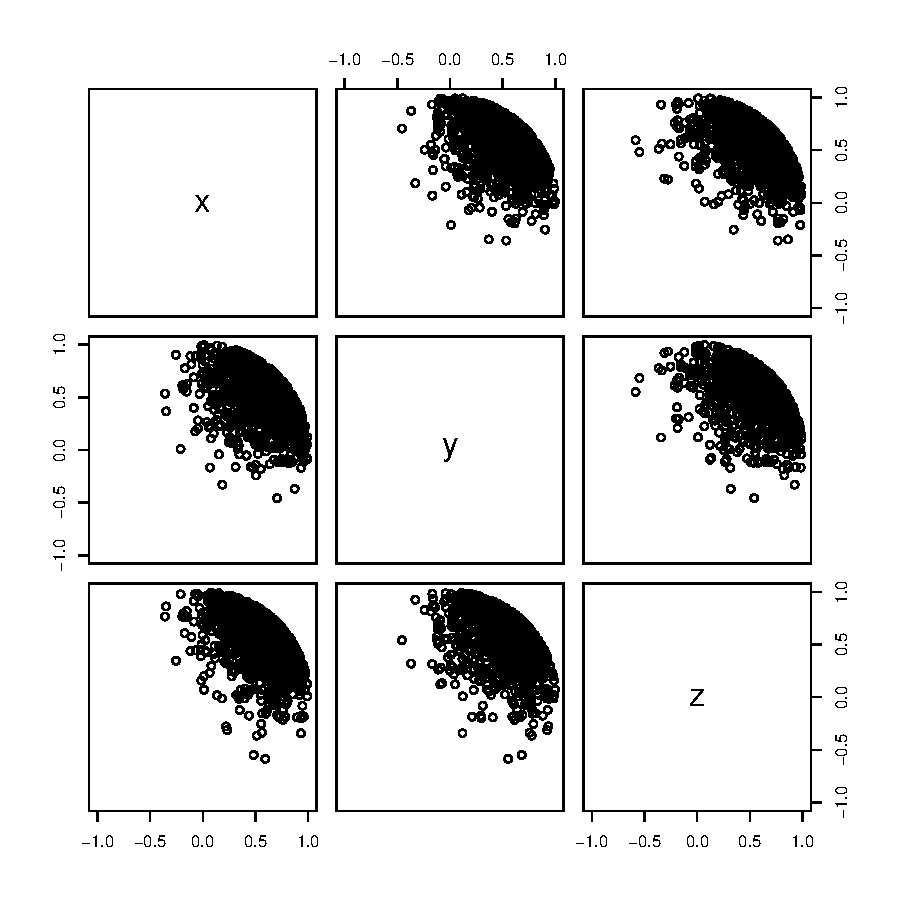
\includegraphics[width=1\textwidth]{sphere_vmf}
\caption{Constrained independent Gaussian distribution}
\end{subfigure}
%\begin{subfigure}[b]{0.30\textwidth}
%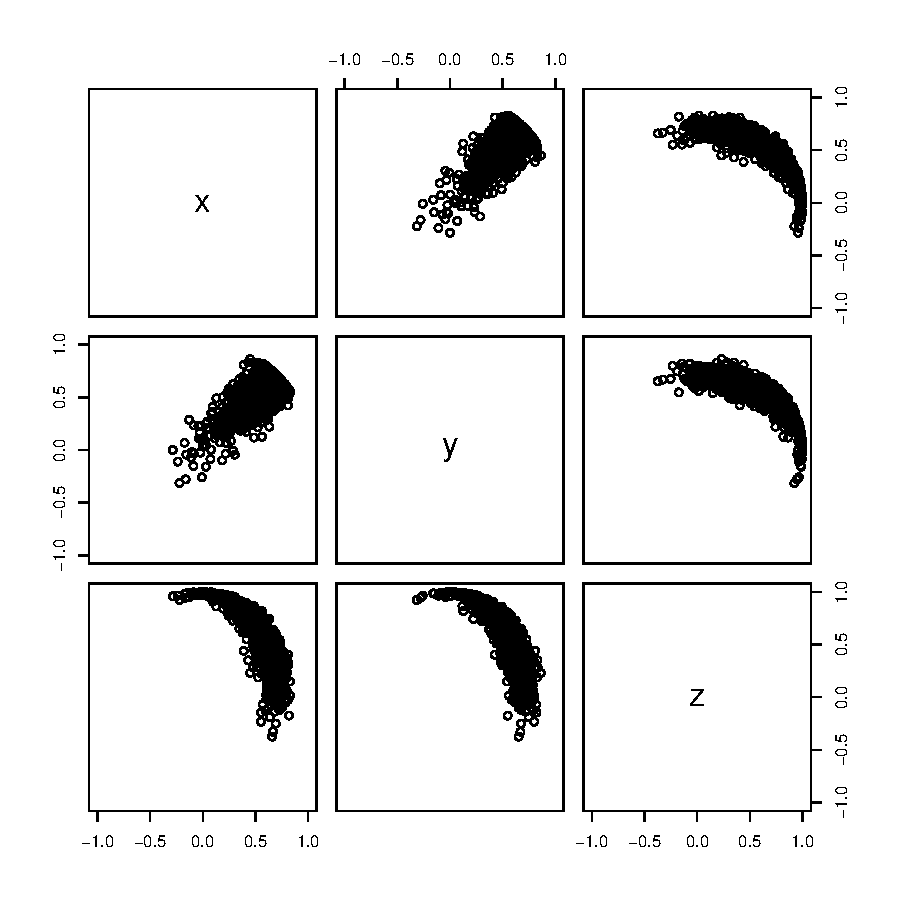
\includegraphics[width=1\textwidth]{sphere_fb}
%\caption{Constrained correlated Gaussian distribution}
%\end{subfigure}
\begin{subfigure}[b]{0.45\textwidth}
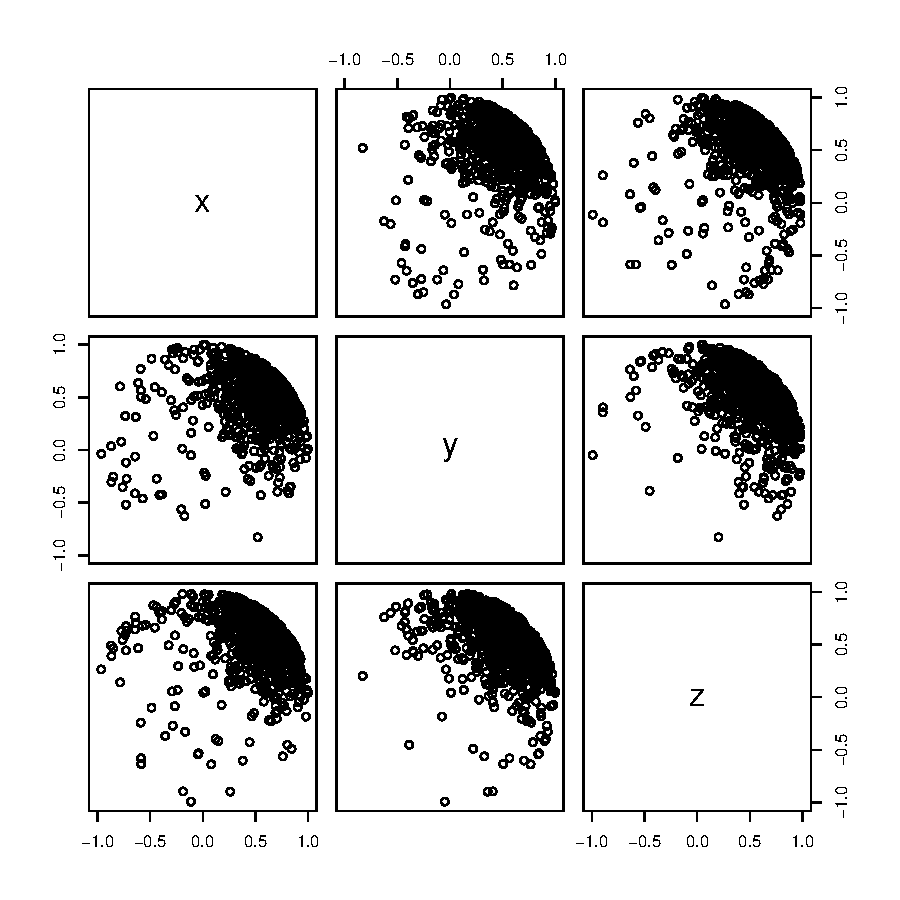
\includegraphics[width=1\textwidth]{sphere_t}
\caption{Constrained independent $t_3$ distribution}
\end{subfigure}
\caption{Sectional view of random samples from constrained distributions on a unit sphere inside $\bb R^3$. The distributions are derived through conditioning on $\theta'\theta=1$ based on unconstrained densities of (a) $\No( F, \diag\{0.1\})$, 
%(b) $\No(F, \left[\protect\begin{smallmatrix} 0.1 & 0.09 & 0 \\ 0.09 & 0.1 & 0 \\ 0 & 0 &0.1  \protect\end{smallmatrix}\right])$,
 (b) $t_3(F,\diag\{0.1\} )$, where $F=[1/\sqrt{3},1/\sqrt{3},1/\sqrt{3}]'$.}
\label{sphere_examples}
\end{figure}

\subsection{ Constraint Relaxation for Posterior Inference}

When the constrained distribution \eqref{constrainedDensity} is used as a prior,
denoting  the likelihood as $ L(y;\theta)$  with $y$ the data, one can obtain posterior:
\be
\label{exactPosterior}
\pi(\theta\mid y) & \propto L(y;\theta)\pi_{\mc D}(\theta) \\
& \propto L(y;\theta) \pi_{\mc
R}(\theta) /J(v(\theta))\mathbbm{1}_{\theta\in \mc D}.
\ee
Clearly, the
posterior also has support only inside $\mc D$ due to the inheritance of
$\mathbbm{1}_{\theta\in \mc D}$ from $\pi_{\mc D}(\theta)$. On the hand,
the indicator is often inconvenient for posterior inference. We now present
present two different strategies to relax the parameter $\theta\in \mc D$ into the neighborhood
of $\mc D$, obtaining posterior $\theta^*$. Then we directly use $\theta^*$ as approximation
or project $\theta^*$ back to $\mc D$ for exact inference. We refer this
strategy as {\bf COnstraint RElaxation (CORE)}.


 \subsubsection{Approximation CORE}

We first present a general approximation strategy. By putting positive mass around $v(\theta)=\bf
0$, and let it decay exponentially, we relax the support of $\theta$ into a
neighborhood surrounding $\mc D $. This generate approximate posterior sample $\theta^*\in \mc R$ via

\be
\label{approximatePosterior}
\tilde{\pi}(\theta^*\mid y)  & = \frac{1}{m(\lambda)} L(y;\theta^*) \pi_{\mc
R}(\theta^*) /J(v(\theta^*)) \exp (- \sum_{k=1}^K |v_k(\theta^*)|^\alpha/\lambda_k),
\ee
where $v_k$ is the $k$th equation in $v(\theta)$, $\alpha$ is
typically chosen as $1$ or $2$ to mimic Laplace or Gaussian kernel, $m(\lambda)$ is an unknown normalizing
constant such that $\int_{\mc R} \tilde{\pi}(\theta^*\mid y) d\theta^*=1$;
 $\lambda_k\ge 0$ is a
tuning parameter controling the concentration around $v(\theta^*)=\bf 0$.
When $\lambda_k=0$ for all $k$, 
\eqref{approximatePosterior} becomes exact; using small $\lambda_k>0$, \eqref{approximatePosterior}
 conventional Monte Carlo approach can be exploited directly.

We use a toy example with closed-form posterior to illustrate the effect of approximation. Consider a posterior from a sum-constrained
bivariate Gaussian random vector $[\theta_1,\theta_2]' \mid y \sim \No(0,I)
\mathbbm{1}_{\theta_1+\theta_2-1=0}$. Using
$v(\theta)=\theta_1+\theta_2-1=0$, $J(v(\theta))=\sqrt 2$, the exact \eqref{exactPosterior} is proportional to 
$$
\phi(\theta_1)
\phi(\theta_2)\mathbbm{1}_{v(\theta)=0}
$$
where $\phi(.)$ is the standard
normal density. The exact posterior density has closed-form

$$
\pi(\theta\mid y)=\frac{\sqrt{2}}{\sqrt{2\pi}} \exp(-\frac{(\theta_1-\frac{1}{2})^2}{2/2})
\mathbbm{1}_{\theta_2=1-\theta_1}
$$
corresponding to $\theta_1\mid (\theta_1+ \theta_2=1) \sim
\No(1/2,1/2)$, $\theta_2\mid \theta_1 \sim \delta_{1-\theta_1}(.)$.
 Marginally, it is a degenerate Gaussian:
$$\begin{bmatrix} \theta_1 \\ \theta_2 \end{bmatrix} \sim
\No_{\text d} \left(
\begin{bmatrix} \frac{1}{2} \\ \frac{1}{2} \end{bmatrix},
\begin{bmatrix} \frac{1}{2} & -\frac{1}{2}  \\  -\frac{1}{2}  & \frac{1}{2} \end{bmatrix}
\right).$$

Using $ \exp( - (\theta^*_1+\theta^*_2-1)^2/\lambda)$ to
replace $\mathbbm{1}_{v(\theta)=0}$, we obtain approximation $\theta^*_1 \sim \No(\frac{2}{\lambda+4},\frac{\lambda+2}{\lambda+4})$, $\theta^*_2\mid \theta^*_1 \sim \No(\frac{2}{\lambda+2}(1-\theta^*_1),\frac{\lambda}{\lambda+2})$. Marginally, 

$$\begin{bmatrix} \theta^*_1 \\ \theta^*_2 \end{bmatrix} \sim
\No \left(
\begin{bmatrix} \frac{2}{\lambda+4} \\ \frac{2}{\lambda+4} \end{bmatrix},
\begin{bmatrix} \frac{\lambda+2}{\lambda+4} & -\frac{2}{\lambda+4}  \\  -\frac{2}{\lambda+4}  &\frac{\lambda+2}{\lambda+4} \end{bmatrix}
\right).$$
As approximation, one can sample from the non-degenerate distribution using small $\lambda$. Clearly, the approximation error decreases as $\lambda$ gets
smaller, and becomes exact when $\lambda\rightarrow 0$. We will formalize
this notion in the theory section.

\subsubsection{Data Augmentation CORE}

The previous strategy is generally applicable. In some less general but
still common cases, one can relax constraint through some function
$g$ first, and there is an inverse function $g^{-1}$ to project it back to
$\mc D$. We now exploit this to reparameterize $\pi_{\mc D}(\theta\mid y)$.

The relaxation $\theta^*=g(\theta;w)$ often requires an auxillary parameter
$w$ independent of $\theta$. Treating $w$ as a latent variable from $\pi(w)$ with $\int_{\mc W} \pi(w) dw =1$ and $\mc W$ as
its support, one uses $g^{-1}(\theta^*;w)$ to reparameterize the exact posterior $\pi_{\mc D}(\theta\mid y)$
Using variable transformation, the density under new parameterization is


\be
\label{reparameterization}
\pi(\theta^*\mid y,w)\pi(w) & =\pi_{\mc D}(g^{-1}(\theta^*;w)\mid y) \frac{1}{J(g(\theta;w))}  \pi(w) \\
&\propto \frac{\pi_{\mc R}(g^{-1}(\theta^*;w)\mid y) }{ J(v(\theta))\mid_{\theta=g^{-1}(\theta^*;w)} } \frac{1}{J(g(\theta;w))} \pi(w) 
\ee
where   $J(g(\theta;w))$ is the Jacobian of $g$ with respect to $\theta$.
The indicator function disappears since $g^{-1}(\theta^*;w)\in \mc
D$ always holds. It can be verified that transforming $\theta^*=g(\theta;w)$  yields $\pi_{\mc D}(\theta\mid y) \pi(w)$, which is the exact posterior augmented
with latent variable $w$. Therefore, we refer this strategy as data augmentation
constraint relaxation (DA-CORE). Using DA-CORE, one can directly sample $\theta^*$ and $w$ in less constrained
space, and apply $\theta=g^{-1}(\theta^*;w)$ in the end to obtain the $\theta$-marginal.

One simple example of relaxation would be scaling of $\theta$ under  norm constraint. For example, $(p-1)$-simplex ,
$\|\theta\|_1=\sum_{i=1}^p\theta_1=1$ with $\theta\in \mc R=[0,\infty]^p$, one
can augment an independent latent variable $w\in [0,\infty)$ have
$\theta_i^*=\theta_i w$, and the inverse $\theta_i=\theta_i^*/w$ with
$w=\|\theta^*\|_1$. Suppose exact posterior is a Dirichlet distribution 
$\theta\mid y\sim \text{Dir}(\alpha)$
, 
$$
\pi_{\mc D}(\theta \mid y)\propto \prod_{i=1}^p \theta_i^{\alpha-1}\mathbbm{1}_{\sum_{i=1}^p\theta_i=1},$$
then the relaxed parameterization is $$
\pi(\theta^*,w\mid y) \propto  \prod_{i=1}^{p-1} (\frac{\theta_i^*}{w})^{\alpha-1}  w^{-(p-1)} \pi(w), \quad w=\sum_{i=1}^p \theta^*_i, \quad \theta^*\in(0,\infty)^p.$$

One can often design the relaxation $g$ if there is a known projection $g^{-1}$ that produces $\theta\in \mc D$. To illustrate, we consider the random variable
$\theta$, a $n$-by-$k$ matrix in the Stiefel manifold $\theta\in \mc V(n,k)=\{\theta\in \bb R^{n\times
k}: \theta'\theta=I\}$, where $n\ge k$. The QR-decomposition produces such
a orthonormal matrix, for which a $n$-by-$k$ matrix $X=QR$,
with $Q\in \mc V(n,k)$ and $R$ $k$-by-$k$ upper triangular and diagonal positive;
 the
QR decomposition is unique if $X$ is of rank $k$ CITES, which allows us to
use it as $g^{-1}$. Letting $w$ be a random matrix, $k$-by-$k$, upper triangular and diagonal positive, we have $\theta^*=\theta w$, with $\theta^*$ in rank
$k$. Suppose $\theta$ is $n$-by-$k$ and from the Matrix Bingham--von Mises--Fisher distribution
\citep{hoff2009simulation},
$$\pi_{\mc D}(\theta\mid y)\propto \text{etr}(C'\theta+B\theta'A\theta)  \mathbbm{1}_{\theta'\theta=I_k}$$
where $\text{etr}$ represents the exponential of trace, $A$ is symmetric $n$-by-$n$, $B$ is symmetric $k$-by-$k$ and $C$ is $n$-by-$k$. The relaxed
parameterization is

$$\pi(\theta^*, w\mid y)\propto \text{etr}(C'\theta^*w^{-1}+B(\theta^*w^{-1})'A\theta^*w^{-1} \text{det}^{-1}(w), \quad \text{rank}(\theta^*)=k, \quad w= \text{QR.R}(\theta^*)$$
where $\text{ QR.R}$ denotes the function that outputs $R$ matrix in QR decomposition.

In other reparameterization, such as coordinate system, one often
needed to use equal or less parameters to satisfy the constraint, which is
often difficult and yields complex parameterization. In DA-CORE, it is generally
easy to reparameterize, since it meets the constraint with more parameters, thanks to data augmentation. Since $w$ is independent of $\theta$, one can
assign $\pi(w)$ to allow greater relaxation, which is commonly associated
with better performance in posterior sampling. More will be illustrated in
the following sections.


 \subsection{Properties}

We now present the properties of the proposed approach. We first establish
that the conditioning approach yields valid probability measure.

We focus on $\mc R$ being a $p$-dimensional Euclidean space and the
intrinsic dimension of $\mc D$, $\mbox{dim}(\mc D)=s\le p$ and is integer.
When $s<p$, although the
$p$-dimensional Lebesgue measure $\mu^p(\mc D)=0$, it is still possible to define a conditional probability given the event ${v(\theta)=\bf 0}$. We utilize the concept of {\it regular
conditional probability} (r.c.p.)
\citep{kolmogorov1950foundations}. For this article to be self-contained,
we list the definition as below (a more complete review can be found in \cite{leao2004regular}).

Let $(X, \mathscr A, \mu)$ be a probability space and $(Y, \mathscr B)$ a measurable space. A function $v$ is measurable if $v:X\rightarrow Y$, $v^{-1}(\mathscr B)\in \mathscr A$.
A r.c.p is a function
$f: Y\times \mathscr A \rightarrow[0,1]$ satisfying:

\begin{enumerate}
        \item $f(y, .)$ is a measure on $(X,\mathscr A)$ for each $y \in
        Y$;
        \item $f(., E)$ is a measurable function on $(Y,\mathscr B)$ for each $E\in \mathscr A$;
        \item For each $E \in \mathscr A$, $F\in \mathscr B$,
        $\mu(E \cap v^{-1}(F))=\int_{F} f(y, E) \mu_y(dy)$, with
        $\mu_y$ the induced measure on $(Y,\mathscr B)$.
\end{enumerate}

Using the previous notation, we write $f(y,E)= P(\theta\in E\mid
v(\theta)=y)=\int_E \pi_{\mc R}(\theta
\mid v(\theta)=y) d\theta$

\begin{remark}
Assuming $J(v(\theta))> 0$ and there is a finite and
non-negative integer $s$ such
that, for some $y\in Y$,
\be
m_s(y)=\int \frac{\pi_{\mc
R}(\theta)
\mathbbm{1}_{v({\theta})=y}}{J(v(\theta))}\mu^s(d\theta)\in(0,\infty),
\ee
then
\begin{equation}
P(E\mid v(\theta)=y)=\left\{\begin{array}{ll}  \frac{1}{m_s(y)}\int_{E } \frac{\pi_{\mc
R}(\theta) \mathbbm{1}_{v({\theta})=y}}{J(v(\theta))}\mu^s(d\theta)
& \text{  , if }m_s(y)\in(0,\infty) \\
\delta_{x^*}(E) \text{ with fixed } x^*\in \bb R^p
& \text{  , if }m_s(y)\in\{0,\infty\} \\
\end{array}\right.
\end{equation}
is a valid r.c.p..
\end{remark}
\begin{proof} The first two crieria for r.c.p are trivally satisfied. Hausdorff measure is the standard tool for geometric measure theory \citep{federer2014geometric}, defined as $\mc H^{s}(A)= \underset{\delta\rightarrow 0}\lim \inf \{ \sum \left[{\text{diam}(S_i)}\right]^s: {A\subseteq \cup S_i, \text{diam}(S_i)\le \delta}, \text{diam}(S_i)=\sup_{x,y\in S}\|x-y\|\}$. We denote the normalized Hausdorff measure as $\bar{\mc H}^{s}(A) =\frac{\Gamma(\frac{1}{2})^{s}}{2^s \Gamma(\frac{s}{2}+1)} \mc H^{s}(A)$. When $s$ is an integer, Lebesgue and normalized Hausdorff measures coincide  $\mu^{s}(A)= \bar{\mc H}^{s}(A)$ \citep{evans2015measure}.

Similar to the proof of (2) of Proposition 2 of \cite{diaconis2013manifold}, using co-area formula \citep{federer2014geometric}:

\be
\mu(E\cap v^{-1}(F))= & \int \mathbbm{1}_{\theta \in E} \mathbbm{1}_{\theta \in v^{-1}(F)}\pi_{\mc R}(\theta)\mu^p(d\theta) \\
= & \int \left[ \int_{v^{-1}(y)} \mathbbm{1}_{\theta \in E} \mathbbm{1}_{v(\theta) \in F}  \frac{ \pi_{\mc R}(\theta)}{J(v(\theta))} \bar{\mc H}^{s}(d\theta)\right] \mu^{p-s}(dy) \\
= & \int_{F} \left [ \int_{ E \cap \bb R^{s}}  \frac{ \pi_{\mc R}(\theta) \mathbbm{1}_{v(\theta)=y}}{J(v(\theta))} \mu^{s}(d\theta)  \right] \mu^{p-s}(dy) \\
\ee


For $y\in \{y':m(y')=0\}$, $\int_{ E}  \frac{ \pi_{\mc R}(\theta) \mathbbm{1}_{v(\theta)=y}}{J(v(\theta))} \mu^s(d\theta) \le \int_{ \bb R^{s}}  \frac{ \pi_{\mc R}(\theta) \mathbbm{1}_{v(\theta)=y}}{J(v(\theta))} \mu^s(d\theta) =0$; for $y\in \{y':m(y')=\infty\}$, since $\mu ^{p}(\bb R^p)=\int \mathbbm{1}_{m(y)=\infty}m(y) dy + \int  \mathbbm{1}_{m(y)<\infty}m(y)  dy=1$, one must have $\int \mathbbm{1}_{m(y)=\infty} dy=0$. Combining parts yields
\be
\mu(E\cap v^{-1}(F)) & = \int_{F} \mathbbm{1}_{m(y)\in (0,\infty)}\left[
\int_{E} \frac{\pi_{\mc
R}(\theta) \mathbbm{1}_{v({\theta})=y}}{J(v(\theta))}
\mu^{s}(d\theta) \right] \mu^{p-s}(dy) \\
& = \int_{F} \mathbbm{1}_{m(y)\in (0,\infty)}
\left[ \int_{E}  \frac{1}{m(y)}  \frac{\pi_{\mc
R}(\theta) \mathbbm{1}_{v({\theta})=y}}{J(v(\theta))}
\mu^{s}(d\theta) \right ]  m(y)\mu^{p-s}(dy)\\
& =\int_F f(y,E) \mu_y(dy) 
\ee

\end{proof}

The above remark gives the definition of r.c.p given all $v(\theta)\in Y$. Since our primary interest is when $v(\theta)=\bf 0$, as long as $m_s({\bf 0})\in (0,\infty)$ at certain integer $s$, we would have a valid conditional density 

\be 
\pi_{\mc D}(\theta)=
\frac{1}{m({\bf 0})}  \frac{\pi_{\mc
R}(\theta) \mathbbm{1}_{v({\theta})={\bf 0}}}{J(v(\theta))}
\ee 

The dimension $s$ is often referred as `intrinsic' dimension of $\mc D$. Formally, one would use a standard concept in geometric measure theory named Hausdorff measure,  \citep{federer2014geometric}. The $d$-dimensional Hausdorff measure is the limit total volume of the $d$-dimenional balls covering $A$, $\mc H^{d}(A)= \underset{\delta\rightarrow 0}\lim \inf \{ \sum \left[{\text{diam}(S_i)}\right]^d: {A\subseteq \cup S_i, \text{diam}(S_i)\le \delta}, \text{diam}(S_i)=\sup_{x,y\in S}\|x-y\|\}$. Then the intrinsic dimension is equal to Hausdorff dimension $s=\inf_{d\ge 0}\{H^d(\mc D)=0\}=\sup_{d\ge 0}\{H^d(\mc D)=\infty\}$, at which the Hausdorff measure transitions from $0$ to $\infty$. Although finding $s$ can be challenging \citep{mardia1975statistics,bowen1979hausdorff}, one could could heuristically test $s\in \{p,p-1,\ldots, 0\}$ if $s$ is known to be an integer. Fortunately, for posterior estimation, there is no need for estimating $s$ or the normalizing constant $m_s(\bf 0)$ in Monte Carlo sampling.

We now quantify the approximation error of the approximate-CORE \eqref{approximatePosterior}. 
We use $\Pi(.)$ and $\tilde\Pi(.)$ to represent the measures under exact and approximating distributions. 
 For easier notation, we re-parameterize the approximating part as $\exp(-\lambda^{-1}  v(\theta))$ where $\lambda=\max_k \lambda_k$ and $v(\theta)=\sum_{k=1}^d\frac{|v_k(\theta)|^{\alpha}}{\lambda^*_k}$ with $\lambda^*_k=\lambda_k/\lambda$ and define a conditional expectation, $\mathbb{E}(g(\theta) \mid v(\theta)=x)=  \int_{\bb R^s } \frac{ g(\theta) \mathbbm{1}_{v(\theta)=x} \pi_{\mc R}(\theta)}{ J v(\theta) } d \theta.$

 We now assess the behavior of approximation error in terms of 1-Wasserstein distance, as $\lambda$ decreases towards $0$. The 1-Wasserstein distance $W_1(\Pi,\tilde\Pi)$ represents the minimal amount of transport needed to transform one distribution to another. Formally, it is defined as

$$W_1(\Pi,\tilde\Pi)=\underset{\gamma\in \Gamma(\Pi,\tilde\Pi)}{\inf}\int \|\theta-\theta^*\| d\gamma(\theta,\theta^*)$$ 
where $\Gamma(\Pi,\tilde\Pi)$ is the family of all joint measures of with $\Pi$ and $\tilde\Pi$ as the marginals, and $\|\theta-\theta^*\|$ is the
Euclidean distance.



%Due to similar form in prior and posterior, we now introduce some general notation. Let $\pi_{\mc R}(\theta)$ be the normalized density in $\mc R$ such that $\int \pi_{\mc R}(\theta)=1$, which is $\pi_{0,\mc R}(\theta)$ for prior and $L(y;\theta)\pi_{0,\mc R}(\theta)$ for posterior;% Suppose $\Phi:\mathbb R^p \rightarrow \mathbb R^d$ with $p>d$ is Lipschitz, then the co-area formula \citep{federer2014geometric} is,
% \begin{equation}
% \ \int_{\mathbb{R}^n}  f(\theta)J_N\Phi(\theta)\mu^n(d \theta)
% =\ \int_{\mathbb{R}^m}  \int_{\Phi^{-1}(y)}f(\theta) \mc H^{n-m}(d\theta)\mu^m(d y),
% \end{equation}
% where $\mu^k(d\theta)$ a $k$-dimensional Lebesgue measure. 


\begin{remark}
The 1-Wasserstein distance between the measures based on \eqref{exactPosterior} and \eqref{approximatePosterior} has
$$ \underset{\lambda \rightarrow 0}\lim W_1(\Pi,\tilde\Pi)=0.$$
Further, for $\alpha=1$ in \eqref{approximatePosterior},

\begin{equation}
\begin{aligned}
W_1(\Pi,\tilde\Pi) \le \lambda (\frac{k_1 k_2}{m(0)^2} + \frac{k_1}{m(0)}) + \exp(- \lambda^{-1} t )(\frac{k_1}{m(0)^2} + \frac{k_3}{m(0)}),
\end{aligned}
\end{equation}
where $k_1=\underset{g:\|g\|_L\le 1}\sup\underset{t^*\in [0,t)}\sup \|\mathbb{E}(g(\theta^*) \mid v(\theta^*)=t^*)\|$, $k_2= \underset{t^*\in (0,t)}\sup  m(t^{*})$ and $k_3=\underset{g:\|g\|_L\le 1} \sup \mathbb{E}(\| g(\theta )\|)$.
\end{remark}


\begin{proof}[Proof]
Let $g:\mathbb{R}^p\rightarrow \mathbb{R}$ be a 1-Lipschitz continuous function, i.e. $\|g(x)-g(y)\|\le \|x-y\|$, denoted by $\|g\|_L\le 1$. 
By Kantorovich-Rubinstein duality, the 1-Wasserstein distance based on Euclidean metric equals to: 

\begin{equation}
W_1(\Pi,\tilde\Pi)=\underset{g:\|g\|_L\le 1}\sup \int g(x) \Pi(dx) -  \int g(y) \tilde\Pi(dy) 
\end{equation}

Taking $g(\theta)=\exp(-\lambda^{-1}v(\theta))$ yields
\begin{equation}
\begin{aligned}
m_\lambda
& = \int_\mathbb{R}  \left[ \int_{v^{-1}(x)} \frac{ \exp(- \lambda^{-1} v(\theta) ) \pi_{\mc R}(\theta)}{ J v(\theta) } \mathcal{H}^{p-d}(d \theta) \right] \mathbbm{1}_{x \ge 0}  d x \\
& = \int_\mathbb{R}  m(x)\exp(- \lambda^{-1} x ) \mathbbm{1}_{x \ge 0}  d x .
\end{aligned}
\end{equation}

Taking $g(\theta)={\mathbbm{1}_{v(\theta)=0}}$ yields 
\begin{equation}
m_0
= \int_\mathbb{R} \left[ \int_{v^{-1}(y)} \frac{ \pi_{\mc R}(\theta) }{ J v(\theta) } \mathcal{H}^{p-d}(d \theta) \right]\mathbbm{1}_{y=0} dy   =  \int_{v^{-1}(0)} \frac{ \pi_{\mc R}(\theta) }{ J v(\theta) } \mathcal{H}^{p-d}(d \theta) =m(0)
\end{equation}


Clearly $m_\lambda \ge m_0$.

1. Asymptotic result:

We have

\begin{equation}                
\label{wass0}
\begin{aligned}
&\underset{g:\|g\|_L\le 1}\sup\int g(\theta)  \left[ \frac{ \exp(- \lambda^{-1} v(\theta)) } {  m_\lambda}  - 
\frac{ \mathbbm{1}_{v(\theta)=0} } {  m_0} 
\right]  \frac{\pi_{\mc R}(\theta)}{Jv(\theta)} \mc H^{p-d}(d \theta) \\
&= \underset{g:\|g\|_L\le 1}\sup\int_\mathbb{R}  \mathbb{E}(g(\theta) \mid x)  \left[ \frac{ \exp(- \lambda^{-1} x) \mathbbm{1}_{x \ge 0}} {  m_\lambda}  - 
\frac{ \mathbbm{1}_{x=0} } {  m_0} 
\right] d x \\
&=      \underset{g:\|g\|_L\le 1}\sup\int_\mathbb{R}  \mathbb{E}(g(\theta) \mid x)  \left[ \frac{  1} {  m_\lambda}  - 
\frac{ 1 } {  m_0} 
\right]\mathbbm{1}_{x=0} d x  + \underset{g:\|g\|_L\le 1}\sup\int_\mathbb{R}  \mathbb{E}(g(\theta) \mid x)\frac{ \exp(- \lambda^{-1} x)} {  m_\lambda}  
\mathbbm{1}_{x > 0} d x \\
& \le \underset{g:\|g\|_L\le 1}\sup \|\mathbb{E}(g(\theta) \mid 0)\| \left[ \frac{ 1 } {  m_0} -\frac{  1} {  m_\lambda}   
\right] + \frac{1} {  m_0} \underset{g:\|g\|_L\le 1}\sup \int_\mathbb{R}  \|\mathbb{E}(g(\theta) \mid x)\| { \exp(- \lambda^{-1} x)}
\mathbbm{1}_{x > 0} d x \\      
\end{aligned}
\end{equation}


Note $m_\lambda\le \int_\mathbb{R} m(x) \mathbbm{1}_{x \ge 0}  dx =\int_\mathbb{R} \pi_{\mc R}(\theta) =1$. By dominated convergence theorem, 

\begin{equation}
\lim_{\lambda\rightarrow 0}m_\lambda= \int_\mathbb{R}  m(x) \lim_{\lambda\rightarrow 0}\exp(- \lambda^{-1} x ) \mathbbm{1}_{x \ge 0}  d x = m_0.
\end{equation}


Since 
$ \underset{g:\|g\|_L\le 1}\sup \int_\mathbb{R}  \|\mathbb{E}(g(\theta) \mid x)\| { \exp(- \lambda^{-1} x)} dx \le \int_\mathbb{R} \underset{g:\|g\|_L\le 1}\sup \|\mathbb{E}(g(\theta) \mid x)\| { \exp(- \lambda^{-1} x)} dx$,
letting $q_\lambda=       \underset{g:\|g\|_L\le 1}\sup \|\mathbb{E}(g(\theta) \mid x)\| { \exp(- \lambda^{-1} x)}
\mathbbm{1}_{x > 0}  $, we have $0\le q_1-q_{\lambda_1}\le q_1-q_{\lambda_2}$ for $1\ge\lambda_1\ge \lambda_2$, by monotone convergence theorem, $\lim_{\lambda\rightarrow 0}\int [ q_1(x)-q_\lambda(x)]dx = \int [q_1(x)- q_0(x) ]dx$ hence $\lim_{\lambda\rightarrow 0}\int q_\lambda(x)dx =0$. Combining the results yields 



\begin{equation}
\underset{\lambda \rightarrow 0}\lim W_1(\Pi,\tilde\Pi)=0.        \end{equation}

2. Non-asymptotic result:


\begin{equation}
\label{wass1}
\begin{aligned}
\frac{1}{m_0}-\frac{1}{m_\lambda} & \le  \frac{   \int_\mathbb{R}  m(x) \exp(- \lambda^{-1} x ) \mathbbm{1}_{x > 0}  d x } {  m_0^2}  \\
&= \frac{1}{ m_0^2} \left[ \int_0^{t}  m(x) \exp(- \lambda^{-1} x ) dx + \int_t^{\infty}  m(x) \exp(- \lambda^{-1} x ) dx \right] \\
&\le \frac{1}{ m_0^2} \left[  \underset{t^*\in (0,t)}\sup m(t^{*})\int_0^{t} \exp(- \lambda^{-1} x ) dx + \exp(- \lambda^{-1} t )\int_t^{\infty}  m(x) dx  \right] \\
&\le \frac{1}{ m_0^2} \left[\lambda \underset{t^*\in (0,t)}\sup  m(t^{*})  + \exp(- \lambda^{-1} t ) \right] 
\end{aligned}
\end{equation}

\begin{equation}
\label{wass2}
\begin{aligned}
& \underset{g:\|g\|_L\le 1}\sup\int_\mathbb{R}  \|\mathbb{E}(g(\theta) \mid x)\| { \exp(- \lambda^{-1} x)}  \mathbbm{1}_{x > 0} d x \\
&\le \underset{g:\|g\|_L\le 1}\sup\underset{t^*\in (0,t)}\sup \|\mathbb{E}(g(\theta) \mid t^*)\|     
\int_0^{t} \exp(- \lambda^{-1} x ) dx + \exp(- \lambda^{-1} t ) \underset{g:\|g\|_L\le 1}\sup \int_t^{\infty}   \|\mathbb{E}( g(\theta )\mid x)\| dx \\
&\le \underset{g:\|g\|_L\le 1}\sup\underset{t^*\in (0,t)}\sup \|\mathbb{E}(g(\theta) \mid t^*)\|     \lambda + \exp(- \lambda^{-1} t ) \underset{g:\|g\|_L\le 1} \sup \mathbb{E}(\| g(\theta )\|) \\
\end{aligned}
\end{equation}

Combining \eqref{wass0}\eqref{wass1}\eqref{wass2}, $k_1=\underset{g:\|g\|_L\le 1}\sup\underset{t^*\in [0,t)}\sup \|\mathbb{E}(g(\theta) \mid t^*)\|$, $k_2=\underset{g:\|g\|_L\le 1} \sup \mathbb{E}(\| g(\theta )\|)$, $k_3= \underset{t^*\in (0,t)}\sup  m(t^{*})$


\begin{equation}
\begin{aligned}
& \underset{g:\|g\|_L\le 1}\sup \int g(x) \Pi(dx) -  \int g(x) \tilde\Pi(dx) \\
        %&\le  \frac{k_1}{ m_0^2} \left[\lambda k_3  + \exp(- \lambda^{-1} t ) \right] 
        %+ \frac{1} {  m_0} [ k_1       \lambda + \exp(- \lambda^{-1} t )k_2 ]\\     
        & \le \lambda (\frac{k_1 k_3}{m_0^2} + \frac{k_1}{m_0}) + \exp(- \lambda^{-1} t )(\frac{k_1}{m_0^2} + \frac{k_2}{m_0})
        \end{aligned}
        \end{equation}


        \end{proof}

        


The first part shows the asymptotic accuracy of the approximation. The second part shows the rate with non-asymptotic $\lambda$ under mild assumptions. The interpretation for these assumptions is that if in a small space expansion of $\mc D$, defined as $\{\theta^*: v(\theta^*)\in [0,t] \}$, the marginal density of $v(\theta^*)$ and the conditional expectation of Lipschitz functions are bounded $k_1,k_2= \mc O(1)$, and the expected norm of Lipschitz function are smaller than a bound that grows near exponentially $k_3 = \mc O(\lambda \exp(t/\lambda))$, then the distance $W_1(\Pi,\tilde\Pi)$ converges to $0$ in $\mc O(\lambda)$ as $\lambda\rightarrow 0$.



\section{Posterior Computation}

Adapting  unconstrained density into space $\mc D$ often disrupts its posterior conjugacy. Since one can sample the posterior directly inside $\mc R$ using
 CORE, one can exploit conventional sampling tools such as slice sampling, adaptive Metropolis-Hastings and Hamiltonian Monte Carlo (HMC). In this section, we focus on HMC for its easiness to use and good performance in block updating of parameters in relatively high dimension.

\subsection{Hamiltonian Monte Carlo under Constraint Relaxation}

We provide a brief overview of HMC for continuous $\theta^*$ under constraint relaxation. Discrete extension is possible via recent work of \cite{nishimura2017discontinuous}. For easy notation, we use $q$ to represent $\theta^*$ under approximation-CORE \eqref{approximatePosterior}, and $\{\theta^*, w\}$ under DA-CORE \eqref{reparameterization}.

In order to sample $q$, HMC introduces an auxillary momentum variable $p \sim \No(0, \mass)$. The covariance matrix $\mass$ is referred to as a \textit{mass matrix} and is typically chosen to be the identity or adapted to approximate the inverse covariance of $q$. HMC then sample from the joint target density $\pi(q, p) = \pi(q) \pi(p) \propto \exp (- H(q, p))$ where, in the case of the posterior under relaxation, 


\begin{equation}
\begin{aligned}
H(q, p)& = U(q)+K(p),\\
\text{where } & U(q) = -\log\pi(q),\\
& K(p) = \frac{p'\mass^{-1} p}{2}.
\end{aligned}
\end{equation}
with $\pi(q)$ is the unnormalized density in \eqref{approximatePosterior} or \eqref{reparameterization}. %$L(\theta^*;y)\pi_{0,\mc R}(\theta^*) \exp( - \sum_k\frac{|v_k(\theta^*)|^\alpha}{\lambda_k}) / J(v(\theta^*))$ based on \eqref{approximatePosterior} and $f(q)= L(g(\theta^*;w);y)\pi_{0,\mc R}(g(\theta^*;w))J(g(\theta^*;w)) / J(v(g(\theta^*;w)))$ based on \eqref{reparametrizedPosterior}. 

From the current state $(q^{(0)},p^{(0)})$, HMC generates a proposal for Metropolis-Hastings algorithm by simulating Hamiltonian dynamics, which is defined by a differential equation:

\begin{equation}
\begin{aligned}
\label{hamiltonian}
\frac{\partial q ^{(t)}}{\partial t} & =\frac{\partial H(q, p)}{\partial p} = \mass^{-1}p,\\
\frac{\partial p^{(t)}}{\partial t}& =-\frac{\partial H(q, p)}{\partial q} = -\frac{\partial U(q)}{\partial q}.
\end{aligned}
\end{equation}

The exact solution to \eqref{hamiltonian} is typically intractable but a valid Metropolis proposal can be generated by numerically approximating \eqref{hamiltonian} with a reversible and volume-preserving  integrator \citep{neal2011mcmc}. The standard choice is the \textit{leapfrog} integrator which approximates the evolution $(q^{(t)},p^{(t)}) \to (q^{(t + \dt)},p^{(t + \dt)})$ through the following update equations:

\begin{equation}
\begin{aligned}
\label{leap-frog}
p \leftarrow p - \frac{\dt}{2} \frac{\partial U}{\partial  q },\quad
q \leftarrow  q  + \dt \mass^{-1}p,\quad
p \leftarrow p -  \frac{\dt}{2}  \frac{\partial U}{\partial  q } 
\end{aligned}
\end{equation}
Taking $L$ leapfrog steps from the current state $(q^{(0)},p^{(0)})$ generates a proposal $(q^{*},p^{*}) \approx (q^{(L \dt)},p^{(L \dt)})$, which is accepted with the probability 
$$1\wedge \exp  \left( - H(q^{*},p^{*}) + H(q^{(0)},p^{(0)}))\right)$$


\subsection{Computing Efficiency and Support Expansion}

Since constraint relaxation expands the support from $\mc D$ to $\mc
R$, it is useful to study the effect of space expansion on the computing efficiency. In this section, we provide some  quantification of the effects and provide a practical guidance on choosing $\pi(w)$ or $\lambda$ in the two constraint relaxation strategies.


In understanding the computational efficiency of HMC, it is useful to
consider the number of leapfrog steps to be a function of $\dt$ and
set $L = \lfloor \tau / \dt \rfloor$ for a fixed integration
time $\tau > 0$. In this case, the mixing rate of HMC is completely
determined by $\tau$ in the limit $\dt \to 0$ \citep{betancourt17}. In
practice, while a smaller stepsize $\dt$ leads to a more accurate
numerical approximation of Hamiltonian dynamics and hence a higher
acceptance rate, it takes a larger number of leapfrog steps and
gradient evaluations to achieve good mixing. For an optimal
computational efficiency of HMC, therefore, the stepsize $\dt$ should
be chosen only as small as needed to achieve a reasonable acceptance
rate \citep{beskos13, betancourt14}. A critical factor in determining
a reasonable stepsize is the \textit{stability limit} of the leapfrog
integrator \citep{neal2011mcmc}. When $\dt$ exceeds this limit, the
approximation becomes unstable and the acceptance rate drops
dramatically. Below the stability limit, the acceptance rate $a(\dt)$
of HMC increases to 1 quite rapidly as $\dt \to 0$ and in fact
satisfies $a(\dt) = 1 - \mc O(\dt^4)$ \citep{beskos13}.

For simplicity, the following discussions assume the mass matrix $\mass$ is taken to be the identity. Let $\hess_U(q)$ denote the hessian matrix of $U(q) = - \log \pi(q)$ and let $\xi_1(q)$ denotes the first largest eigenvalue of $\hess_U(q)$. While analyzing stability and accuracy of an integrator is highly problem specific, the linear stability analysis and empirical evidences suggest that, for stable approximation of Hamiltonian dynamics by the leapfrog integrator in $\bb R^p$, the condition $\dt < 2\xi_1(\theta)^{-1/2}$ must hold on most regions of the parameter space \citep{hairer06}.
Besides the eigenvalue, if the support of $q$ is a constrained space $\mc Q$, another limiting factor is roughly the shortest distance to the boundary $\eta (\theta; {\mc Q})= \inf_{q'\not\in \mc Q}\|q'-q\|$. If either $\eta (\theta; {\mc Q})$ or $\xi_1(\theta)^{-1/2}$ 
is close to $0$, the upper bound would be too low to obtain efficient computation.
In constrained model, the parameter space $\mc D$ can have very small $\eta(\theta;\mc D)$. Constraint relaxation can reduce this problem as it provides support
expansion. 

For approximation-CORE \eqref{approximatePosterior}, to minimize approximation
error, one can choose to relax a subset of constraints. Observing  $\mc D=\cap_{k} D_k$,
each approximation $\exp(-\frac{|v_k(\theta^*)|^\alpha}{\lambda_k})$ corresponds to a constrained space $\mc D_k$.  One practical strategy is that, for $\mc D_k$'s with $\eta(\theta;\mc D_k)\approx 0$, one uses moderate $\lambda_k$ to induce some support expansion (denoted by $\lambda_k\ge \zeta$ with $\zeta$ moderately small but not too close to $0$);  for $\mc D_k$'s without this issue, one uses very small $\lambda_k\approx 0$ to almost always uphold the constraint.
The latter was also suggested by \cite{neal2011mcmc} as creating a high `energy wall'. This could create  inaccuracy of HMC near the boundary with $\lambda_k\approx 0$ under fixed step size, therefore we use random step size $\epsilon$ at each iteration.


The Hessian $\hess_U(q)$ under approximation-CORE is given by
\begin{equation}
\label{eq:hessian_extrinsic}
\hess_U(q) = -\hess_{\log L(y;\theta^*) \pi_{\mc
R}(\theta^*) /J(v(\theta^*)) }(\theta^*)+\sum_k \lambda_k^{-1} \hess_{|v_k|^\alpha}(\theta^*) \mathbbm{1}_{\theta\not\in \mc D_k},
\end{equation}
where the second term $\lambda_k^{-1} \hess_{v_k}(\theta) \mathbbm{1}_{\theta\not\in \mc D_k}$ is $0$ unless $\theta\not\in \mc D_k$. Since the $\lambda^{-1}_k$'s
in the second term often dominate the eigenvalue, hence $\xi^{-1/2}_1(\theta^*)\approx
\underset{\lambda_k\ge \zeta}{\min}\lambda_k^{1/2}$. A trade-off between approximation accuracy and computational efficiency is involved. Fortunately, the approximation error $\mc O( \underset{\lambda_k\ge \zeta}{\max}\lambda_k)$ decreases faster than the efficiceny cap $\mc O( \underset{\lambda_k\ge \zeta}{\min}\lambda_k^{1/2})$. In our experiment, we did find changing from $\lambda_{k}=10^{-4}$ to $10^{-5}$ requires approximately $3$ times of computing budget, due the effect on stability
bound.


On the other hand, since DA-CORE \eqref{reparameterization} does not involve such trade-off, it can be more preferrable despite its less
general application. Letting $\mc Q_\theta\subset \mc D$ denote the support for the constrained $\theta\in \mc D$, the reparameterization changes the support to $Q_{\theta^*}=\{g(\theta;w):\theta\in \mc Q\}$. Therefore, one could choose $\pi(w)$ to substantially increase $\eta(\theta^*; Q_{\theta^*})$.
Since the augmented variable $w$ is independent from $\theta$, DA-CORE can
be considered as a parameter expansion  \citep{liu1999parameter}, which originally
focused on accelerating  Gibbs sampling of probit regression. Although  it is possible to use diffuse or even improper prior for $\pi(w)$ on $Q_{\theta^*}$,
 we recommend assigning $\pi(w)$ loosely centered at $w_0:g(\theta;w_0)=\theta$ (corresponding to $\theta^*=\theta$), which makes $\theta^*$ a mild relaxation of $\theta$
and ensures no substantial change in $\xi^{-1/2}_1(\theta^*)$ in HMC.

\section{Simulations}
In order to compare with existing approaches on computing efficiency and provide empirical evidence
supporting our previous result, we run simulations on several toy examples
 in this section.
   
\subsection{Gaussian  under Linear Inequality}
We first consider linear models under linear inequality constraints. Although
recent work proposed a new class of prior with posterior conjugacy \citep{danaher2012minkowski} , one can simply use Gaussian prior under our framework. We sample a bivariate Gaussian $\theta \sim \No \left( \mu, I\sigma^2\right)$ subject to linear inequality $\theta\in(0,1)^2,\theta_1+\theta_2<1$,
which is a triangle. In two separate settings, choosing $(\mu, \sigma^2)$ as $([0.3,0.3],1/{10})$  induces a wide-spread distribution centered in the interior of $\mc D$, while $([0.7,0.3]',1/10^4)$  induces a  distribution concentrated on the boundary of $\mc D$. We use the approximation-CORE  \eqref{approximatePosterior} with $\exp(-\frac{|v(\theta)|}{\lambda})$, with $v(\theta)=|\theta_1+\theta_2-1|_+ + |-\theta_1|_+ + |-\theta_2|_ + + |\theta_1-1|_+ + |\theta_2-1|_+$.  Since the triangle has $\eta(\theta;\mc D)$ away from $0$, small $\lambda=10^{-8}$
 allows almost no approximation error. Figure~\ref{linear_inequality} plots the posterior sample and its contour. To compare, we ran simple rejection sampling with untruncated normal proposal $\No ( \mu, I\sigma^2)$. It  suffers from a rapidly growing rejection rate from $12\%$ to $51\%$, as $\mu$ moves further away from the center of $\mc D$.

\begin{figure}[H]
\begin{subfigure}[b]{0.45\textwidth}
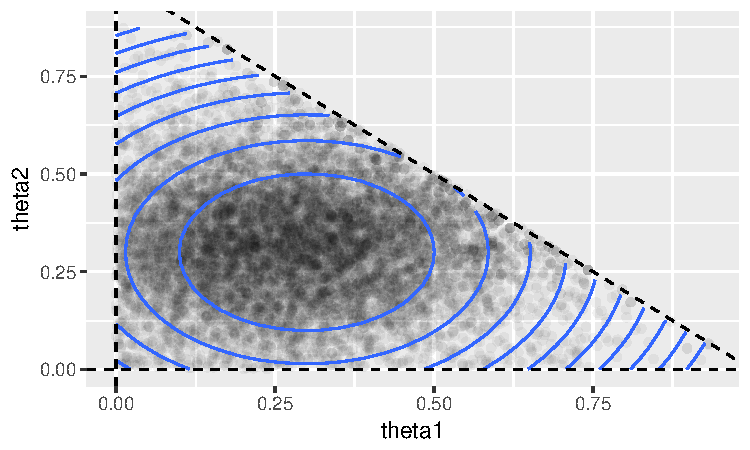
\includegraphics[width=1\textwidth]{linear_inequal_1}
\caption{Constrained $\No([0.3,0.3],1/{10})$}
\end{subfigure}
\begin{subfigure}[b]{0.45\textwidth}
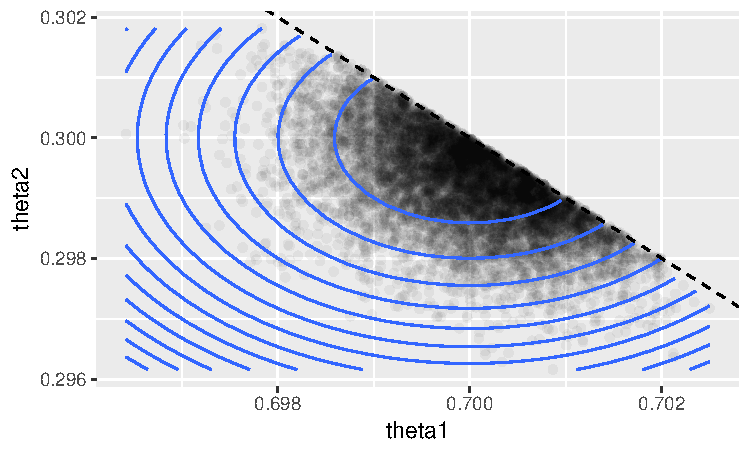
\includegraphics[width=1\textwidth]{linear_inequal_2}
\caption{Constrained $\No([0.7,0.3],1/{10^4})$}
\end{subfigure}
\caption{Posterior sample of bivariate normal distribution subject to linear inequality constraints $\theta\in(0,1)^2,\theta_1+\theta_2<1$, using HMC with  constraint relaxation. Posterior is spread out around the center (panel (a)) or concentrated on the boundary (panel (b)) of the region.}
\label{linear_inequality}
\end{figure}

\subsection{von Mises--Fisher on Unit Circle}
To illustrate equality constraint relxation, we generate a simple von Mises--Fisher distribution $\pi_{\mc D}(\theta) \propto \exp(F'\theta)$ on a unit circle $\{(\theta_1,\theta_2):\theta_1^2+\theta_2^2=1\}$. We use $F=(5,5)$ to induce a relatively spreaded-out  $\theta$ on the manifold.
For sampling,
we compare three strategies: approximate-CORE using $\exp(-\frac{|\theta'\theta -1|}{\lambda})$ for approximating the indicator, DA-CORE
using $\theta_1 = \frac{\theta_1^*}{w}, w= \sqrt{(\theta_1^*)^2+ (\theta_2^*)^2}$ and $\pi(w)\sim \No(1,1)\mathbbm{1}_{w>0}$ and  exact  von Mises--Fisher obtained using `movMF' package.

Unlike the previous linear inequality constraint, the unit circle has narrow
$\eta(\theta;\mc D)=0$ for all $\theta\in \mc D$, therefore, some support expansion is needed
for HMC. We test $\lambda = 10^{-3}$, $10^{-4}$ and $10^{-5}$ for approximation-CORE. To compare the efficiency of HMC, we fix the number of leap-frog steps to $20$ within one iteration HMC, and let software STAN
automatically tune for stable step size. Table~\ref{table_circle} shows the effective sample size per $1000$ iterations, the effective `violation' $|v(\theta)|=|\theta_1+\theta_2-1|$ and the 1-Wasserstein distance $W_1$ as the approximation error. As $W_1$ is numerically computed, to provide a baseline error, we also calculate the average $W_1$ comparing two independent samples from the same exact distribution. The approximation error $W_1$ based on $\lambda= 10^{-5}$ approximation is indistinguishable from this low numerical error, while the other approximations  have slightly larger error but more effective samples. As expected, the DA-CORE is exact
and has high effective sample size. 
   \begin{table}[H]
   \begin{center}
   \tiny
   \begin{tabular}{ c| c | c| c |c | c}
   \hline     
    & \multicolumn{4}{c|}{ HMC based on CORE}     & Exact  \\   
       \hline     
        & \multicolumn{3}{c|}{Approximation}     & DA-CORE  \\           
       \hline           
     &  $\lambda=10^{-3}$ & $\lambda=10^{-4}$ & $\lambda=10^{-5}$ &  
     &  \\
   \hline
   \hline
   $W_1$ & 0.050 & 0.034  & 0.014 & 0.017  & 0.015 \\

   &  (0.019, 0.095) &(0.027, 0.037) &  (0.013,0.025)  & (0.0012,0.026) & (0.0014,0.025)\\

   \hline
   $|v(\theta)| \mid y$ 
   & $9\times 10^{-4} $ 
   & $9\times 10^{-5} $ 
   & $9\times 10^{-6} $ &0 & 0\\
   & $(2.6 \cdot 10^{-5}, 3.3\cdot 10^{-3})$& $(2.0 \cdot 10^{-6}, 3.4\cdot 10^{-4})$& $(2.7 \cdot 10^{-7}, 3.5\cdot 10^{-5})$&  & \\
   \hline
   ESS /1000 Iterations &  751.48  & 260.54 & 57.10 & 788.30    \\
   \hline  
   \end{tabular}
   \end{center}
   \caption{Benchmark of constraint relaxation methods on sampling von--Mises Fisher distribution on a unit circle. For each approximation CORE, average approximation error (with 95\% credible interval, out of $10$ repeated experiments) is computed, and numeric error of $W_1$ is shown under column `exact' as comparing two independent copies from the exact distribution.\label{table_circle}.
Effective sample size shows DA-CORE and approximation-CORE with relatively large $\lambda$ have high computing efficiency.
}
   \end{table}

\subsection{Dirichlet on a Simplex}
Lastly, we experiment with a particularly challenging distribution on a 
$(p-1)$-simplex, defined by $\{\theta: \theta\in(0,\infty)^p,\sum_{i=1}^p \theta_i=1\}$. We consider Dirichlet distribution $\text{Dir}(\alpha)$, with
$\pi_{\mc D}(\theta)\propto \prod_{i=1}^p\theta_i^{\alpha-1}$. When the concentration
parameter $\alpha<1$, $\text{Dir}(\alpha)$ exhibits sparse property that some $\theta_i$'s become very close to $0$, which is exploited in many modeling
approaches CITES. Despite the simple form, the computation can be quite difficult
 if there is large uncerntainty associated with $\theta$ on top of sparsity.
 The distribution will be multi-modal with distribution scattered along the boundary of the simplex (Figure~\ref{simplex}(a)).

To illustrate, we consider $p=3$ and various values of $\alpha\in \{1,0.5,0.1,0.01\}$. We test the performance of approximation-CORE and DA-CORE. To compare, we also test the standard HMC using coordinate
system $\theta_1=\cos^2(\theta_1^*), \theta_2=\sin^2(\theta_1^*)\cos^2(\theta_2^*), \theta_3=\sin^2(\theta_1^*)\sin^2(\theta_2^*)$ for $\theta^*\in [0,2\pi)^2$,
which is equivalent to stick-breaking representation CITES; and the geodesic
HMC utilizing the geometric flow directly on the simplex \citep{byrne2013geodesic}.
For all HMCs, we fix the number of steps in each iteration to be $30$ and tune the step size to have the best effective sample size.

Table~\ref{simplex_tb} lists the effective sample sizes under different $\alpha$'s.
As $\alpha$ becomes smaller than $1$, approximation-CORE and geodesic HMC become worse in performance, while DA-CORE
 and coordinate system are much less impacted.
Figure~\ref{simplex}(b) shows at $\alpha=0.01$, the approximation-CORE and geodesic
HMC are stuck for a long time, while DA-CORE works substantially better. As a well-tested reparameterization,  HMC based on coordinate system still works acceptably well in this case.

The difficulty that approximation-CORE encountered was  anticipated. \cite{byrne2013geodesic} have previously reported similar
slow-down of geodesic HMC computing on hyper-Dirichlet  distribution CITES with $\alpha<1$. Comparing these two approaches, geodesic HMC relies on restricting the kinetic flow on $\mc D$ via its product with the metric tensor, and approximation-CORE relies
on creating high energy wall in the potential energy part. The latter can
be as an approximation
to the former, which explains the similarity in performance.


\begin{figure}[H]
\begin{subfigure}[b]{0.45\textwidth}
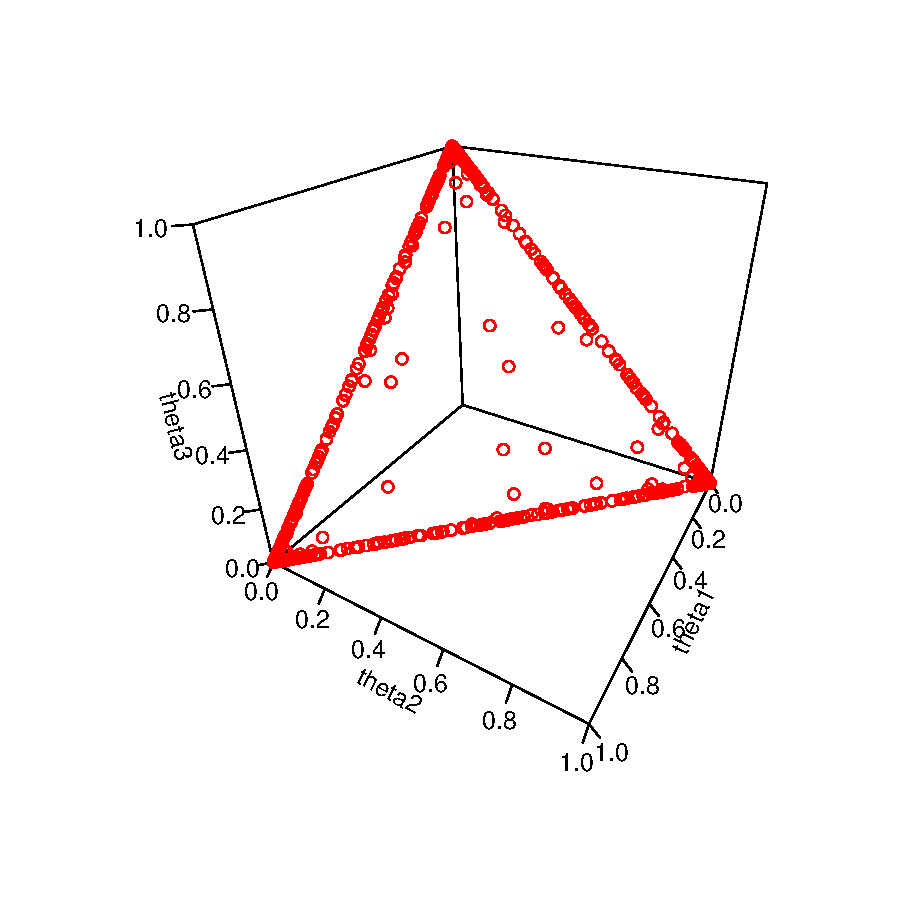
\includegraphics[width=1\textwidth]{simplex001}
\caption{$2,000$ samples from $\text{Dir}(0.01)$ on $2$-simplex.}
\end{subfigure}
\begin{subfigure}[b]{0.45\textwidth}
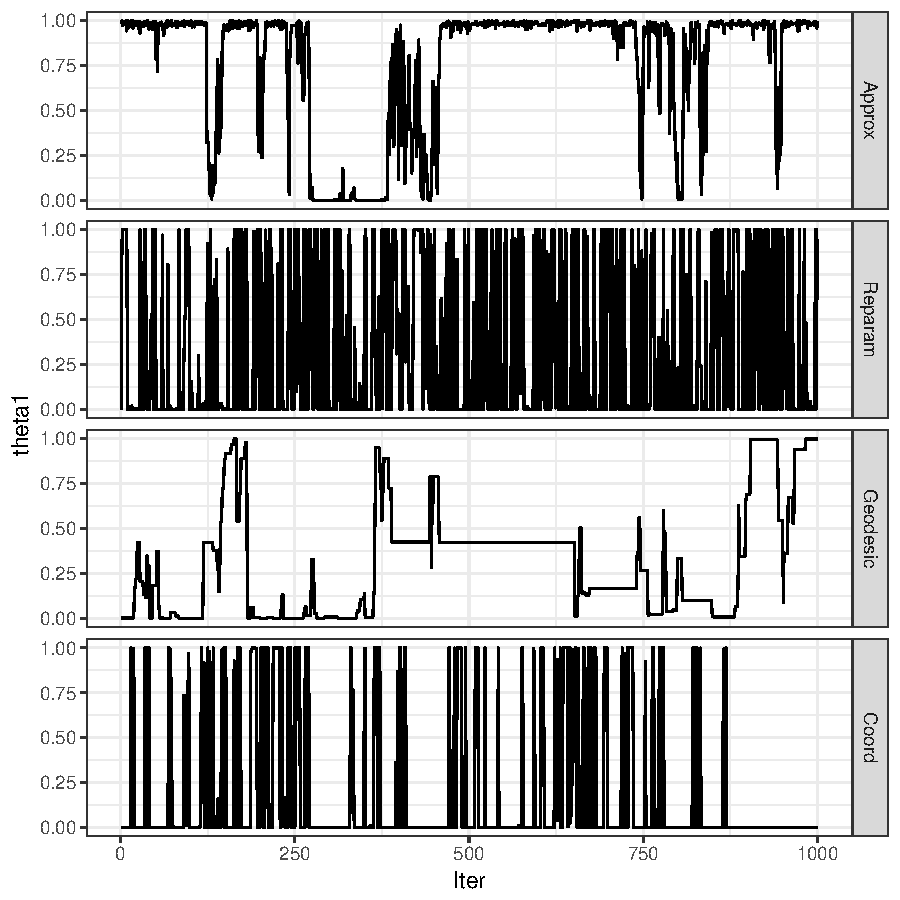
\includegraphics[width=1\textwidth]{simplexTrace001}
\caption{Traceplot of $\theta_1$ using 4 types of HMCs.}
\end{subfigure}
\caption{Sampling of Dirichlet on an simplex with distribution concentrated on the boundaries.
Panel(a) illustrates the distribution under $\text{Dir}(0.01)$; Panel(b)
compares the traceplots of 4 different types of HMCs, which are based on: approximation-CORE with $\lambda=10^{-3}$, DA-CORE, geodesic flow on simplex \citep{byrne2013geodesic} and coordinate
system.}
\label{simplex}
\end{figure}


   \begin{table}[H]
     
   \begin{center}
   \tiny
   \begin{tabular}{ l| r | r| r |r | r}
   \hline     
    & \multicolumn{3}{c|}{HMC based on CORE}     & Geodesic HMC  & Coord
    System HMC \\   
        & {Approx $\lambda=10^{-3}$} & {Approx $\lambda=10^{-4}$}      & DA
        &  \\  \hline         
   ESS /1000 Iter. ($\alpha=1$) & 511.43   & 146.07  & 947.53 &  174.14
   & \bf 961.08     \\
      ESS /1000 Iter. ($\alpha=0.5$) & 145.15  & 33.16  &\bf  912.94  & 31.47  & 846.92   \\
            ESS /1000 Iter. ($\alpha=0.1$) &  88.32   & 26.88& \bf 992.75  &28.70  & 875.83    \\
   ESS /1000 Iter. ($\alpha=0.01$) & 20.54 & 3.91 & {\bf 722.44} & 17.26  & 128.55  \\
   \hline  
   \end{tabular}
   \end{center}
   \caption{Average effective sample size per $1000$ iterations in $\text{Dir}(\alpha)$,
   under different $\alpha$. \label{simplex_tb}
}
   \end{table}

   \section{Application: Sparse Basis Learning in Network Analysis}

 We now consider a real data application in brain network analysis. 
 The brain connectivity structures are obtained in the data set KKI-42 (Landman et al. 2011), which consists of $n=21$ healthy subjects without any history of neurological disease. We take the first scan out of the scan-rescan data
as the input. Each observation is a $V\times V$ symmetric network $A_i$, recorded as adjacency matrix $A_i$ for $i=1,\ldots,n$. The regions are constructed via the Desikan et al. (2006) atlas, for a total of V = 68 nodes.
For the $i$th matrix $A_i$, $A_{i,k,l} \in \{0,1\}$ is the element on the $k$th row and $l$th column of $A_i$, with $A_{i,k,l}=1$ indicating there is an connection betwen $k$th and $l$th region, $A_{i,k,l}=0$ if there is no connection. The matrix is symmetric due to the undirectedness of the network,
but the diagonal records $A_{i,k,k}$ for all $i$ and $k$ are missing due
to the lack of meaning in self-connectivity. For this reason, in addition
to the sample size $n$ much smaller
than the ambient space $p=\frac{V(V-1)}{2}$, a probabilistic Bayesian model can be parituclarly
useful for uncertainty quantification.

One scientific interest in neuroscience is to identify the important regions
(nodes) in the formation of the average brain network. Although probabilistic
principal component analysis (PPCA) are routinely used for  extracting the first few important bases, it does not selectively identify the important nodes. To
achieve this goal, one natural way is to apply shrinkage on the elements
of principal components.


Geometrically, the principle components denoted by $\{U_1,\ldots,U_d\}$ reside on a Stiefel manifold $\mc V(d,n)=\{U: U'U=I_d\}$, where $U=[U_1,\ldots,U_d]$ is the $n\times d$ matrix. Using $r$ to index $1,\ldots,d$, each $U_r$ represents a $(n-1)$-hypersphere. Applying shrinkage forces some of its sub-coordinates to be close to $0$, which
is approximately reducing $U_r$ to a lower-dimensional hyper-sphere.
Although there was previous work using sparse PCA \citep{zou2006sparse} on
continuous outcome, little work has been done on a probabilistic model for
binary outcome.



For shrinkage, we utilize the double Pareto prior \citep{armagan2013generalized} as unconstrained distribution
$\pi_{\mc R}$ and adapt it onto Stiefel manifold via \eqref{constrainedDensity}. For simplicity, we consider a probabilistic PCA model with a random intercept ,

   \begin{equation*}
   \begin{aligned}
   & A_{i,k,l} \sim \text{Bern}( \frac{1}{1+ \exp(-\psi_{k,l}- Z_{i})})\\
   & \psi_{k,l} = \sum_{r=1}^{d}  v_{r} u_{k,r} u_{l,r}  \\
   & U'U=I \text{ with } U=\{u_{k,r}\}_{k=1,\ldots,n; r=1,\ldots,d}\\
   & \pi(u_{k,r})  \propto  \frac{1}{2(1+ |u_{k,r}|)^{2}} \\
   & Z_{i} \sim \No(0,\sigma^2_z), \quad  \sigma^2_z \sim \text{IG}(2,1)
   \\
   & v_{r} \sim \No(0,\sigma^2_v), \quad  \sigma^2_v \sim \text{IG}(2,1)
   \end{aligned}
   \end{equation*}
   for $k>l$, $k=2,\ldots, V$, $i=1,\ldots,n$. We adapt $\pi_{\mc R}(u)$ as the standard double Pareto prior \citep{armagan2013generalized}, to avoid
dealing with the normalizing constant due to constraint; $Z_i$ is a scalar
used as random intercept; for scale parameter, we
choose weakly informative prior inverse Gamma $\text{IG}(2,1)$, as appropriate for the scale under the logistic link.

   This model is a special Tucker decomposition with a sparse core tensor, whose diagonal plane is equal to $D$ and $0$ for other elements. The Tucker decomposition is more flexible than another routinely used decomposition, namely parallel factor analysis (PARAFAC). The PARAFAC assumes all ranks are equal and the core tensor $D$ only has non-zero value when all its sub-indices are equal. In this case, PARAFAC would assume $d_1=d_2$. The additional flexibility in the Tucker is appealing, as one could utilize the varying rank over different sub-direction (mode) of the tensor. On the other hand, a completely unconstrained Tucker decomposition is not identifiable in the matrices and core tensor, due scaling. For example, one can multiply a $d_1\times d_1$ non-zero diagonal matrix $R$, to $U$ and obtain $U^*=UR$ obtain $D^{*}_{.,r_2,.}=R^{-1}D_{.,r_2,.}R^{-1}$ for $r_2=1,\ldots,d_2$. This leaves the likelihood unchanged, creating identifiability issue. 

   Therefore, we consider applying some constraint on the Tucker decomposition. Motivated by high-order singular value decomposition, we impose orthonormality constraints $U'U=I_{d_1}$ and $W'W=I_{d_2}$. \cite{hoff2016equivariant} previously obtained conjugated posterior for Tucker decomposition under orthonormality constraint, however, the symmetry in undirectedness of networks breaks the conjugacy.

   We assign normal prior for $U_{k,r_2}\sim \No(0,\phi_{1})$, $W_{i,r_1}\sim \No(0,\phi_2)$, $Z_{k,l}\sim \No(0,\phi_3)$, $D_{r_1,r_2}\sim No(0, \phi_{4,r_1,r_2})$ for all $i,k,l,r_1,r_2$, and inverse-Gamma prior $\phi_1,\phi_2,\phi_3\stackrel{indep}{\sim} \text{IG}(2,1)$, $\phi_{4,r_1,r_2}= \tau_{r_1}\tau_{r_2}$, with $\tau_{r_1},\tau_{r_2}\stackrel{indep}{\sim} \text{IG}(2,1)$ for all $r_1,r_2$. We

%we assign multiplicative inverse gamma distribution \citep{bhattacharya2011sparse} $\phi_{4,r_1,r_2}= \prod_{m_1=1}^{r_1} \nu_{1,m_1} \prod_{m_2=1}^{r_2}  \nu_{2,m_2}$ with $\nu_{1,1},\nu_{2,1} \stackrel{indep}{\sim} \text{IG}(a_1,1)$ and $\nu_{1,m},\nu_{2,m}\stackrel{indep}{\sim} \text{IG}(a_2,1)$ for $m\ge 2$. This induces increasing concentration toward zero as $r_1,r_2$ increase, allowing adaptive choosing of latent dimensions. We set $a_1=a_2=5$ in this application.

To allow estimation for model with orthonormality constraint, we use extrinsic prior with $\mc K(\theta) = \exp( - \frac{(U'U-I_{d_1})^2 + (W'W-I_{d_2})^2  }{\lambda})$ and set $\lambda=10^{-3}$. To compare, we also test with the same model configuration without the orthonormality constraint. We run both models for $10,000$ steps and discard the first $5,000$ steps. Figure~\ref{tucker} plots the traceplot and autocorrelation for matrix $U$. Unconstrained base model has severe convergence issue due to the non-identifiability, while constrained model converges and show low autocorrelation for all the parameters.

\begin{figure}[H]
\begin{subfigure}[b]{1\textwidth}
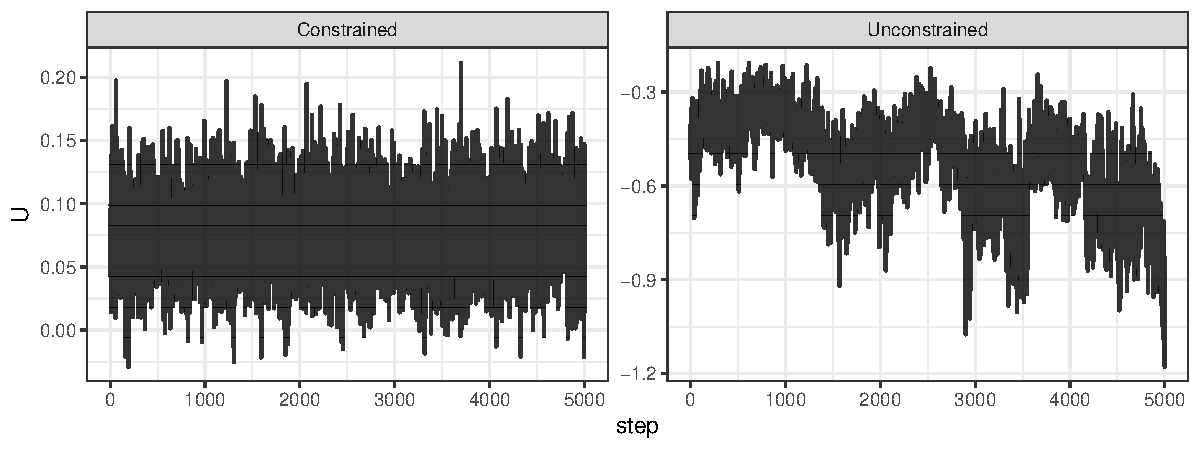
\includegraphics[width=1\textwidth]{tucker_traceplot.pdf}
\caption{Traceplot of $U_{1,1}$.}
\end{subfigure}
\begin{subfigure}[b]{1\textwidth}
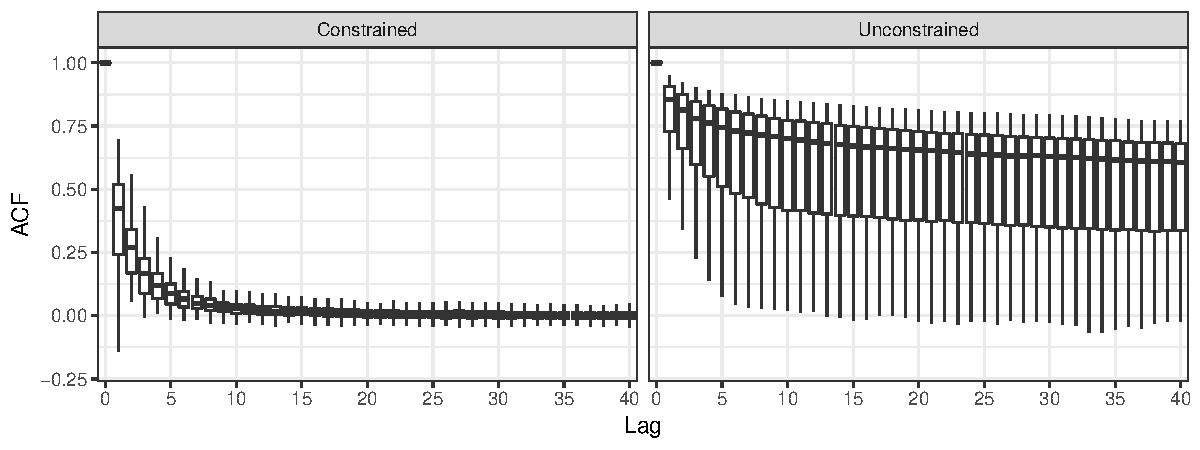
\includegraphics[width=1\textwidth]{tucker_acf.pdf}
\caption{ACF of all elements in $U$}
\end{subfigure}
\caption{Orthonormality constraint in the tensor decomposition modelallows convergence and rapid mixing on the factor matrix (left column); whereas unconstrained model does not converge due to free scaling. Traceplot for one parameter in factor matrix $U$ and boxplot for autocorrelations of all parameters are shown.}
\label{tucker}
\end{figure}

\section{Discussion}

The estimation difficulty associated with parameter constraint often hinders the development of new models. Often one needed to carefully avoid models without conjugate posteriors, or skillfully re-parameterize the model for a more tractable algorithm. The extrinsic approach we introduced significantly reduces the burden. Through space expansion, it allows conventional toolbox such as HMC to be easily adopted to sample posterior without closed-forms. This allows researchers to impose constraints more freely in modeling and simplifies the way to incorporate constraint information about the functional of parameters.

We show the approximation error of the extrinsic approach can controlled via tuning parameter, with some trade-off between computing time and accuracy. A potentially more efficient strategy would be obtaining a rough approximate first in $\mc R$, then projecting into $\mc D$. \cite{lin2016extrinsic} developed algorithms similar to this idea and obtained consistency result for point estimation. A useful task would be to find an optimal projection also quantifying the uncertainty associated with finite sample. Lastly, the normalization of parameters over constrained space can sometime yield intractable integral, known as `doubly stochastic' problem. We expect that the proposed extrinsic prior can be adapted and used together with the various existing solutions \citep{rao2016data,stoehr2017noisy}.



\bibliography{reference}
\bibliographystyle{chicago}
\end{document}


